%*****************************************
\chapter{Hypothesis Testing: Nonparametric Tests}\label{hyp:nonparametric}
%*****************************************
\section{Introduction}

An important function for statistical analysis is to test a hypothesis to see if it adequately explains some observed phenomenon. The statistical processes for qualitative data are introduced in this lab and the processes for quantitative data are in \nameref{hyp:parametric} on \pageref{hyp:parametric}.\footnote{The definitions of ``hypothesis'' and the various data types are found in the \nameref{int:introduction}, beginning on page \pageref{intro:Hypothesis}.} 

\section{Kruskal-Wallis H}

\textit{More Than 2 Groups : Ordinal/Nominal Data : Not Paired}

This test is used to determine if there are any significant differences in three or more groups of ordinal or nominal data. Imagine that a researcher wanted to determine if there was a significant difference in the birth weight for babies born to women who were divided into three groups: ``Heavy Smokers'' (more than one pack per day), ``Light Smokers'' (one pack or less per day), and ``Nonsmokers.'' The researcher would record the birth weights and mothers' smoking habits for all babies born in a single hospital for six months and then use a Kruskal-Wallis H test to see if there was a significant difference in those three groups.

\section{Wilcoxon Signed Ranks} 

\textit{2 Groups : Ordinal/Nominal Data : Paired}

This test is used to determine if there are any significant differences in two groups of paired ordinal or nominal data. ``Paired'' data means that a single data point is observed two different times and those two observations are compared. Imagine that a researcher wanted to know if a speech from the company president could change workers' opinions. The researcher would ask a group of volunteers their opinion about a controversial policy both before and after that speech. The researcher would use a $ 1 $-to-$ 5 $ point scale with questions like ``I would vote for this policy.'' Later, the researcher would compare each person's before/after rating with a Wilcoxon Signed Ranks test to see if there was a significant change in opinion. In this case, the data are paired such that the before/after opinion for each volunteer is compared. 

\section{Mann-Whitney U} 

\textit{2 Groups : Ordinal/Nominal Data : Not Paired}

This test is used to determine if there are any significant differences in two groups of unpaired ordinal or nominal data. Imagine that a movie producer wanted to know if there was a difference in the way the audience in two different cities responded to a movie. As the audience members left the theater they would be asked to rate the movie on a scale of one to five stars. The ratings for the two cities would be collected and then a Mann-Whitney test would be used to determine if the difference in ratings between the cities was significant. 

\section{Procedure}

\texttt{SOFA} makes it easy to complete any of the statistical tests listed in this lab exercise. A Wizard provides help in selecting an appropriate test but users can also manually select and configure whatever test they need.

\subsection{Statistics Wizard}

If the type of data and the question being asked is known then \texttt{SOFA} includes a Wizard to help select an appropriate statistics test. To access the wizard, open \texttt{SOFA} and select ``Statistics.'' Then click ``Or Get Help Choosing Below.''

\begin{itemize}
  \item \textbf{Tests that show if there is a difference.}
  
  \begin{itemize}

    \item \textbf{Groups}. Select the number of groups that are being analyzed: \textit{$ 2 $} or \textit{$ 3 $ or more}. For help in determining how many groups are in the data click the ``Groups'' button near the bottom of the window to open the frequency table function\footnote{See Lab \ref{fre:frequency_tables} on page \pageref{fre:frequency_tables} for more information about frequency tables.} Also, the ``Help'' button to the right of the Groups selection provides good information.

    \item \textbf{Normal}. Select whether the data are in a normal distribution\footnote{See Section \ref{int:normal_distribution} on page \pageref{int:normal_distribution} for more information about the normal distribution.}. For help in determining if the data are normal, click the ``Normality'' button near the bottom of the window. Also, the ``Help'' button to the right of the Normal selection provides good information.

    \item \textbf{Independence}. Select whether the data are independent observations or paired. 

  \end{itemize}

  \item \textbf{Tests that show if there is a relationship.}
  
  \begin{itemize}
  
    \item \textbf{Data Type}. Select ``Names'' if the data are nominal and ``Ordered'' if Ordinal. For help in determing the data type, click the ``Data Type'' button near the bottom of the window. Also, the ``Help'' button to the right of the Data Type selection provides good information.
    
    \item \textbf{Normal}. (Note: this selection is only active for ``Ordered'' data) Select whether the data are in a normal distribution\footnote{See Section \ref{int:normal_distribution} on page \pageref{int:normal_distribution} for more information about the normal distribution.}. For help in determining if the data are normal, click the ``Normality'' button near the bottom of the window. Also, the ``Help'' button to the right of the Normal selection provides good information.
    
  \end{itemize}  
    
\end{itemize}

As an example, the \textit{births} dataset contains information about $ 1000 $ births in North Carolina in $ 2004 $. Imagine that a researcher proposed this hypothesis: ``The weight of babies born to smokers is less than the weight of babies born to nonsmokers.'' The null hypothesis would be ``Smoking makes no difference in the birth weight of babies.'' To test that hypothesis, the researcher would:

Start \texttt{SOFA} and select ``Statistics.'' Then:

\begin{enumerate}
  \item Click ``Or Get Help Choosing Below''
  \item Click ``Tests that show if there is a difference'' since the hypothesis states that smoking causes a difference in birth weight.
  \item The researcher proposes comparing two groups: smokers and nonsmokers. However, to be certain that the dataset does not include any other types of groups (like ``former smokers''), the researcher clicks the ``Groups'' button and the ``Make Report Table'' window opens.\footnote{The creation and use of Frequency Tables are covered in \nameref{fre:frequency_tables} on page \pageref{fre:frequency_tables}.} The researcher creates a frequency table for ``Habit'' and finds that there are only two groups: nonsmoker and smoker.
  
  \begin{figure}[H]
    \begin{center}
      \fbox{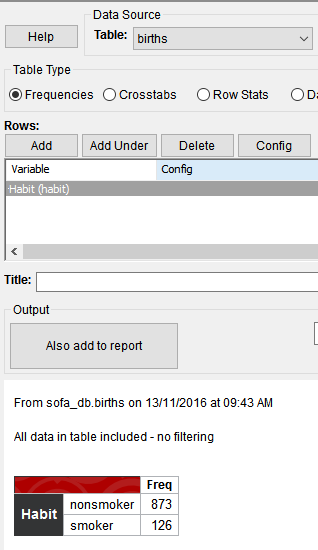
\includegraphics[]{gfx/hypnon005}}
      \caption{Verifying Groups}
    \end{center}
  \end{figure}

  \item Having verified that there are two groups, the researcher must next determine if the birth weight is normally distributed. To do that, the researcher clicks then ``Normality'' button at the bottom of the window. In the ``Normal Data?'' window that pops up, the variable ``weight'' is selected and the following is returned by \texttt{SOFA}:

  \begin{figure}[H]
    \begin{center}
      \fbox{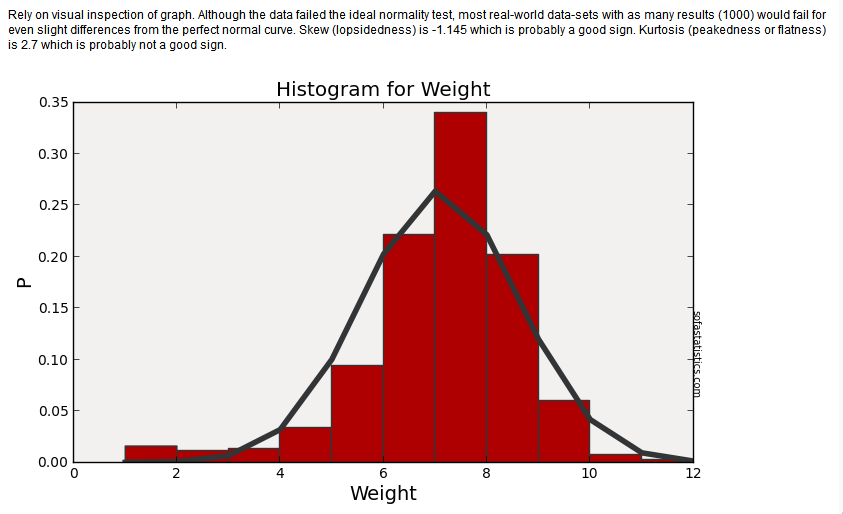
\includegraphics[width=\linewidth]{gfx/hypnon010}}
      \caption{Verifying Normality}
    \end{center}
  \end{figure}

  \item The text above the histogram reports ``Rely on visual inspection of graph. Although the data failed the ideal normality test, most real-world data-sets with as many results ($ 1000 $) would fail for even slight differences from the perfect normal curve. Skew (lopsidedness) is $ -1.145 $ which is probably a good sign. Kurtosis (peakedness or flatness) is $ 2.7 $ which is probably not a good sign.'' In this case, there are $ 1000 $ birth weights recorded so the skew and kurtosis numbers need to tempered by the visual appearance of the histogram. Since the histogram shows a large center peak with ``shoulders'' on both sides this data can be treated as normally distributed.
  \item Next, the researcher must determine if the data are independent observations or paired. In this case there is no pairing indicated so the researcher chooses ``Independent.''
  
  \begin{figure}[H]
    \begin{center}
      \fbox{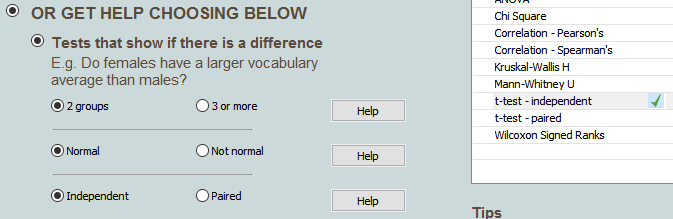
\includegraphics[width=\linewidth]{gfx/hypnon015}}
      \caption{Choosing The Correct Statistical Test}
    \end{center}
  \end{figure}

  \item \texttt{SOFA} indicates that ``t-test - independent'' is the correct test for the data being analyzed, so the researcher clicks the ``Configure Test'' button at the top right corner of the window and proceeds to execute that test. All of the various statistical tests in SOFA are described on the following pages of this lab.

\end{enumerate}

\subsection{Activity 1: Wizard} \label{nonpara:act01}

Using the various settings for the Wizard, what type of test is recommended for the following types of data? Note: in the Word document submitted for this lab, Activity $ 1 $ should have a simple listing, something like this (Note: these are not the correct answers to the listed tests):

\rowcolors{1}{}{}
\begin{center}
  \begin{tabular}{ll}
    $ 1 $ & Mann-Whitney U \\ 
    $ 2 $ & t-test - paired \\ 
    $ 3 $ & Kruskal-Wallis H \\ 
  \end{tabular} 
\end{center}

Here are the three types of data being analyzed:

\rowcolors{1}{gray!25}{}
\begin{center}
  \begin{tabular}{llllll}
    \hline 
    \textbf{No.} & \textbf{Test Type} & \textbf{Groups} & \textbf{Distribution} & \textbf{Indep} & \textbf{Cat} \\ 
    \hline 
    $ 1 $ & Difference & $ 4 $ & Normal & N/A & N/A \\     
    $ 2 $ & Difference & $ 2 $ & Not Normal & Paired & N/A \\     
    $ 3 $ & Relationship & N/A & Normal & N/A & Ordered \\     
    \hline 
  \end{tabular} 
\end{center}

\subsection{Chi Square}

The Chi Square statistic is covered in Lab \ref{cor:chi_square}, \nameref{cor:chi_square}, page \pageref{cor:chi_square}. The \texttt{SOFA} activity related to Chi Square is on page \pageref{cor:chi_square_proc}.

\subsection{Correlation - Spearman's}

The Spearman's Rho statistic is covered in Lab \ref{cor:spearmans_rho}, \nameref{cor:spearmans_rho}, page \pageref{cor:spearmans_rho}. The \texttt{SOFA} activity related to Spearman's Rho is on page \pageref{cor:spearmans_rho_proc}.

\subsection{Kruskal-Wallis H}

\begin{enumerate}
  \item Start \texttt{SOFA} and click the "Statistics" button.
  \item Select "Kruskal-Wallis H" from the Statistical Test list at the top of the window and then click the "Configure Test" button.
  \item Data Source Table: email
  \item Averaged Variable: Dollar. This is the key difference between a Kruskal-Wallis H test and an ANOVA. The Kruskal-Wallis H test expects the ``averaged'' variable to be a non-normal distribution, like ordinal or nominal data, while the ANOVA test expects the ``averaged'' variable to be a normal distribution, like ratio or interval.
  \item Group By Variable: ``Spam''.
  \item From Group: No
  \item To: Yes
  
  \begin{figure}[H]
    \begin{center}
      \fbox{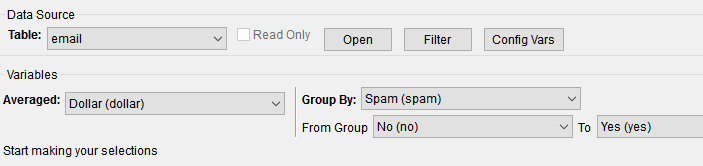
\includegraphics[width=\linewidth]{gfx/hypnon020}}
      \caption{Setting Up a Kruskal-Wallis H Test}
    \end{center}
  \end{figure}
  
  \item The results of that test are found in the results window:
  
  \begin{figure}[H]
    \begin{center}
      \fbox{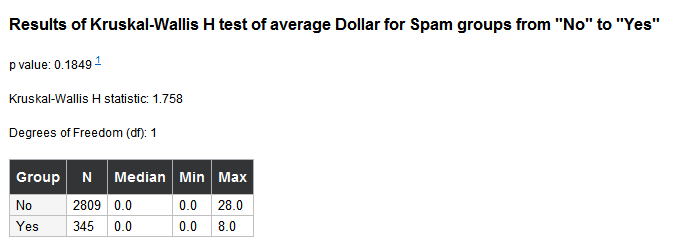
\includegraphics[width=\linewidth]{gfx/hypnon025}}
      \caption{Results of a Kruskal-Wallis H Test}
    \end{center}
  \end{figure}

  \item \textbf{p Value}. The most important statistic in the results window is the p-value. As always, when this number is encountered it is desired for it to have a value less than $ 0.05 $ ($ 5\% $). In the example calculated for this exercise, the p-value is $ 0.1849 $, which is greater than $ 0.05 $, so there is no significant relationship between Dollar and Spam in this dataset.
  \item \textbf{Kruskal-Wallis H statistic}. If the Kruskal-Wallis H statistic is greater than the Chi Square calculated value for the same input variables then the null hypothesis can be rejected. In a separate operation, the Chi Square statistic was calculated as $ 112.033 $ for Dollar and Spam. Since the Kruskal-Wallis H statistic was less than the Chi Square then the null hypothesis could not be rejected. This agrees with the p-value calculated and, in general, if a p-value is available it should be used rather than rely on calculating and comparing to the Chi Square statistic.
  \item \textbf{Others}. All other statistics displayed in the Kruskal-Wallis H results window have been explained elsewhere and will not be further detailed here.
  \item \textbf{Another Example}. As another example, following is a Kruskal-Wallis H test for ``Attach'' and ``Spam.'' Notice that the p-value is $ 4.587 \times 10^{-5} $, which is much less than the threshold of $ 0.05 $, so there is a significant relationship between the number of attachments to an email message and whether that message is spam.
  
  \begin{figure}[H]
    \begin{center}
      \fbox{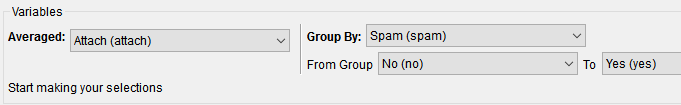
\includegraphics[width=\linewidth]{gfx/hypnon030}}
      \caption{Setting Up a Kruskal-Wallis H Test}
    \end{center}
  \end{figure}

  \begin{figure}[H]
    \begin{center}
      \fbox{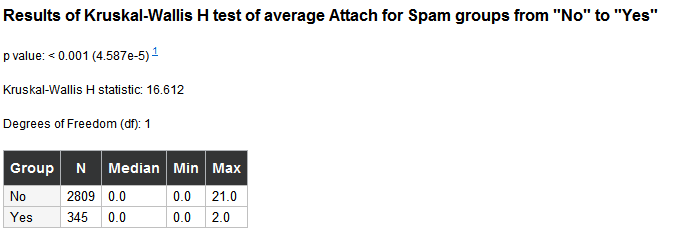
\includegraphics[width=\linewidth]{gfx/hypnon035}}
      \caption{Results of a Kruskal-Wallis H Test}
    \end{center}
  \end{figure}
  
\end{enumerate}

\subsection{Activity 2: Kruskal-Wallis H} \label{nonpara:act02}

Using the \textit{maincafe} dataset in \texttt{SOFA} conduct a Kruskal-Wallis H test and report the \textit{p-value} for the following variables. Note: in the Word document submitted for this lab, Activity $ 2 $ should have a simple listing, something like this. (Notes: these are not the correct answers to the listed tests. To indicate tiny values use scientific notation in a form like $ 1.6e-5 $ since that is easier to type.)

\rowcolors{1}{}{}
\begin{center}
  \begin{tabular}{ll}
    $ 1 $ & $ 0.35 $ \\ 
    $ 2 $ & $ 1.27e-8 $ \\ 
    $ 3 $ & $ 237.4 $ \\ 
    $ 4 $ & $ 0.73 $ \\ 
  \end{tabular} 
\end{center}

Here are the variables to test:

\rowcolors{1}{gray!25}{}
\begin{center}
  \begin{tabular}{cllll}
    \hline 
    \textbf{Num} & \textbf{Averaged} & \textbf{Group By} & \textbf{From} & \textbf{To} \\ 
    \hline 
    $ 1 $ & Ptysize & Recmd & No & Yes \\ 
    $ 2 $ & Food & Meal & Breakfast & Other \\ 
    $ 3 $ & Bill & Day & Friday & Wednesday \\ 
    $ 4 $ & Tip & Sex & Female & Other \\ 
    \hline 
  \end{tabular} 
\end{center}

\subsection{Mann-Whitney U}

\begin{enumerate}
  \item Start \texttt{SOFA} and click the "Statistics" button.
  \item Select "Mann-Whitney U" from the Statistical Test list at the top of the window and then click the "Configure Test" button.
  \item Data Source Table: email
  \item Ranked Variable: Attach
  \item Group By Variable: Spam
  \item Group A: No
  \item Group B: Yes
  
  \begin{figure}[H]
    \begin{center}
      \fbox{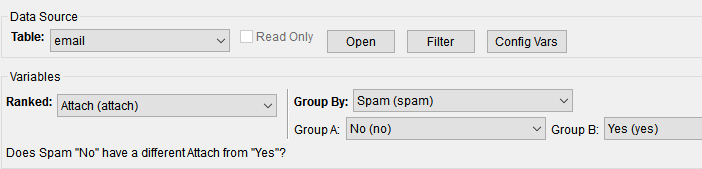
\includegraphics[width=\linewidth]{gfx/hypnon040}}
      \caption{Setting Up a Mann-Whitney U Test}
    \end{center}
  \end{figure}

  \item The results are shown in the figure below.

  \begin{figure}[H]
    \begin{center}
      \fbox{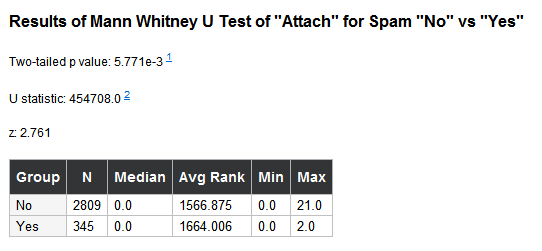
\includegraphics[width=\linewidth]{gfx/hypnon045}}
      \caption{Results of a Mann-Whitney U Test}
    \end{center}
  \end{figure}
    
  \item \textbf{Two-tailed p value}. This is the p-value calculated by the test. The designation of ``two-tailed'' indicates that there were only two groups being analyzed, but the p-value calculated is interpreted exactly the same as for any other test. In this case, since $ 5.771 \times 10^{-3} $ is less than $ 0.05 $ then there is a significant difference in the ``No'' and ``Yes'' spam groups.
  \item \textbf{U Statistic}. This number is of little value except, perhaps, to compare the results of one Mann-Whitney U test to another. The most important result of a Mann-Whitney test is the p-value.
  \item \textbf{z}. A Z-score is a representation of a score as a standard deviation above or below zero. For example, a Z-score of $ 1.0 $ indicates that the score is one standard deviation above zero. In the example calculated for this exercise, the Z-score is $ 2.761 $ which is more than two standard deviations higher than the mean and would indicate that the test results are significant.
  \item \textbf{Other Statistics}. The other statistics presented in a Mann-Whitney U test are routine calculations explained elsewhere.
  
\end{enumerate}

\subsection{Activity 3: Mann-Whitney U} \label{nonpara:act03}

Using the \textit{maincafe} dataset in \texttt{SOFA} conduct a Mann-Whitney U test and report the \textit{p-value} for the following variables. Note: in the Word document submitted for this lab, Activity $ 3 $ should have a simple listing, something like this. (Notes: these are not the correct answers to the listed tests. To indicate tiny values use scientific notation in a form like $ 1.6e-5 $ since that is easier to type.)

\rowcolors{1}{}{}
\begin{center}
  \begin{tabular}{ll}
    $ 1 $ & $ 0.35 $ \\ 
    $ 2 $ & $ 1.27e-8 $ \\ 
    $ 3 $ & $ 237.4 $ \\ 
    $ 4 $ & $ 0.73 $ \\ 
  \end{tabular} 
\end{center}

Here are the variables to test:

\rowcolors{1}{gray!25}{}
\begin{center}
  \begin{tabular}{cllll}
    \hline 
    \textbf{Num} & \textbf{Ranked} & \textbf{Group By} & \textbf{From} & \textbf{To} \\ 
    \hline 
    $ 1 $ & Ptysize & Meal & Breakfast & Other \\ 
    $ 2 $ & Ptysize & Pref & Booth & Table \\ 
    $ 3 $ & Svc & Sex & Female & Other \\ 
    $ 4 $ & Food & Day & Friday & Wednesday \\ 
    \hline 
  \end{tabular} 
\end{center}

\subsection{Wilcoxon Signed Ranks}

\begin{enumerate}
  \item Start \texttt{SOFA} and click the "Statistics" button.
  \item Select "Wilcoxon Signed Ranks" from the Statistical Test list at the top of the window and then click the "Configure Test" button.
  \item Data Source Table: tutoring
  \item Group A Variable: Expgrapre
  \item Group B Variable: Expgra01
  
  \begin{figure}[H]
    \begin{center}
      \fbox{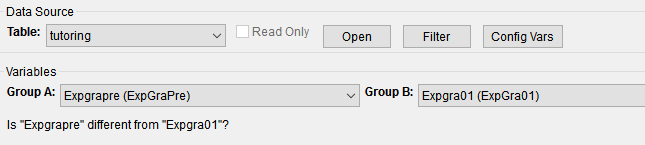
\includegraphics[width=\linewidth]{gfx/hypnon050}}
      \caption{Setting Up a Wilcoxon Signed Ranks Test}
    \end{center}
  \end{figure}
  
  \item \texttt{SOFA} calculates the following result.
  
  \begin{figure}[H]
    \begin{center}
      \fbox{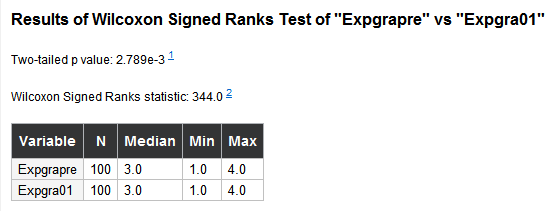
\includegraphics[width=\linewidth]{gfx/hypnon055}}
      \caption{Results of a Wilcoxon Signed Ranks Test}
    \end{center}
  \end{figure}
  
  \item \textbf{p-Value}. As in all other statistical tests, the goal is a p-value less than $ 0.05 $ ($ 5\% $). In the example calculated for this exercise, the p-value is $ 2.789\times10^{-3} $, which is well below the $ 0.05 $ threshold, so the null hypothesis would be rejected.
  \item \textbf{t Statistic}. This number is of little value except, perhaps, to compare the results of one paired t-Test to another. In general, the greater the t-statistic the more likely the null hypothesis can be rejected, but it is challenging to find an appropriate ``cutoff'' score. Therefore, the most important result of an paired t-Test is the p-value.
  \item \textbf{Degrees of Freedom}. This is calculated as the number of observations minus one. Thus, $ 99 $ degrees of freedom indicate $ 100 $ observations in the dataset.
  \item \textbf{Other Statistics}. \texttt{SOFA} also calculates a number of statistics for each of the two groups, but those values are discussed elsewhere and will not be further covered here.
  
\end{enumerate}

\subsection{Activity 4: Wilcoxon Signed Ranks} \label{nonpara:act04}

Using the \textit{maincafe} dataset in \texttt{SOFA} determine if there is a significant difference in the rating customers awarded for food and service (labeled ``svc''). Report the p-value for these two variables.

\section{Deliverable}

Complete the following activities in this lab:

\rowcolors{1}{gray!25}{}
\begin{center}
  \begin{tabular}{lll}
    \hline 
    \textbf{Number} & \textbf{Name} & \textbf{Page} \\ 
    \hline 
    \ref{nonpara:act01} & \nameref{nonpara:act01} & \pageref{nonpara:act01} \\ 
    \ref{nonpara:act02} & \nameref{nonpara:act02} & \pageref{nonpara:act02} \\ 
    \ref{nonpara:act03} & \nameref{nonpara:act03} & \pageref{nonpara:act03} \\ 
    \ref{nonpara:act04} & \nameref{nonpara:act04} & \pageref{nonpara:act04} \\ 
    \hline 
  \end{tabular} 
\end{center}

Consolidate the responses for all activities into a single document and submit that document for grading.


